\documentclass{article}
\usepackage[utf8]{inputenc}
\usepackage{graphicx}
\usepackage[polish]{babel}
\usepackage[T1]{fontenc}

\title{sprawozdanie}
\author{Maksymilian Szewczyk}
\date{December 2022}

\begin{document}

\maketitle

\section{Wprowadzenie teoretyczne.}

Spadek swobodny to ruch, który odbywa się wyłacznie pod wpływem ciężaru, czyli siły grawitacji, bez oporów powietrza. Jego przykładem jest ruch planet wokół Słońca. Kinetyczne równanie ruchu \ref{równanie 1}:

\begin{equation}
\label{równanie 1}
    h(t) = h_0 - \frac{gt^2}{2}
\end{equation}    


gdzie h(t) to wysokość na jakiej znajduje się ciało po czasie t, 

$h_0$ to wysokość z jakiej spada ciało, a t to czas spadania.

\vspace{5mm} %5mm vertical space

źródło: https://pl.wikipedia.org/wiki/Spadek.swobodny

\section{Opis eksperymentu.}

Schemat wykonania doświadczenia przedstawiony jest na rysunku \ref{spadek.swobodny}.

\begin{figure}[htbp]
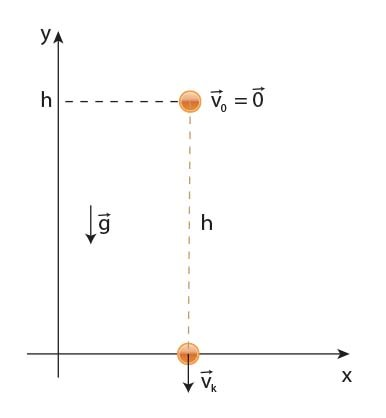
\includegraphics[width=6cm]{zdj.jpg}
\centering
\caption{Spadek swobodny.}
\label{spadek.swobodny}
\end{figure}

\vspace{5mm} %5mm vertical space
źródło: https://www.medianauka.pl/spadek-swobodny 

\section{Wyniki pomiarów}

Wyniki pomiarów przedstawione są na wykresie 1 oraz w tabeli 1.

\section{Wnioski.}

Wszystkie ciała w polu grawitacyjnym spadają z takim samym przyspieszeniem.

\end{document}
